\documentclass[a4paper,12pt]{article} % добавить leqno в [] для нумерации слева

\usepackage{lab_preamble}

\begin{document}

\LabTitle{1.2.3}{Определение моментов инерции твердых тел с помощью трифилярного подвеса}

\textbf{Цель работы}:
\begin{enumerate}
  \item измерение момента инерпии ряда тел и сравне-ние результатов с расчетами по теоретическим формулам
  \item проверкааддитивности моментов инерции и справедливости формулы Гюй-тенса-Штейнера.
\end{enumerate}

\textbf{Приборы}:
\begin{enumerate}
\item трифилярный подвес
\item секундомер
\item счетчик числа колебаний
\item набор тел (диск, стержень, полый цилиндр и другие)
\end{enumerate}

\section{Краткая Теория.}

\begin{equation}
  I = \int_{V}{r^2 dm} \label{eq:1}
\end{equation}
где I - момент инерции тела, r - расстаяние точечной массы тела dm до оси врациния.

\begin{figure} [h] \center
  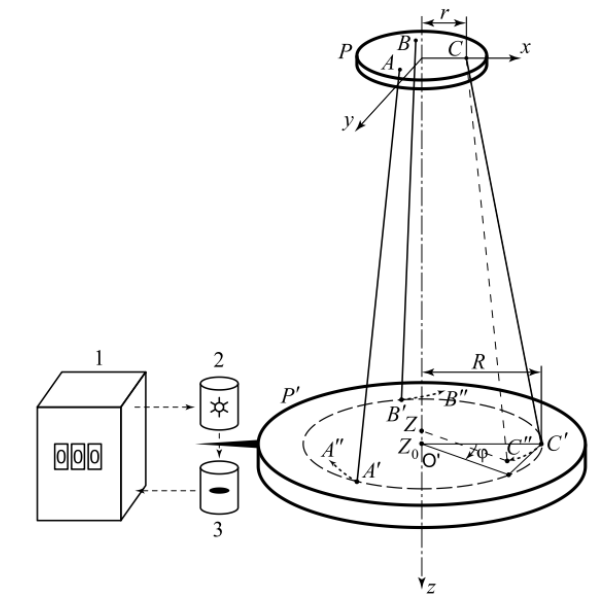
\includegraphics[scale = 0.6]{123/рис 1.png}
  \label{pic:1} \caption[Рис. 1]{Трифилярный подвес}
\end{figure}

Для однородных тел известной плотности при заданных размерах и достаточно простой форме момент инерции можно вычислить. Для неоднородных тел и тел сложной формы момент инерции можно определить экспериментально. Удобно использовать устройство, показанное на рис. \ref{pic:1} и называемое трифилярным подвесом. Оно состоит из укрепленной на некоторой высоте неподвижной платформы Р и подвешенной к ней на трех симметрично расположенных нитях АА’, ВВ'и СС' вращающейся платформы Р'.
Платформа Р укреплена на кронштейне и снабжена рычагом, при помощи которого в системе можно создать крутильные колебания путем небольшого поворота верхней платформы. (Лучше поворачивать верхнюю платформу)
В результате платформа будет совершать крутильные колебания.

Если пренебречь потерями энергии на трение, то ЗСЭ можно записать следующим образом:
\begin{equation}
  \frac{I \dot{\varphi^2}}{2} + mg(z_0 - z) = E \label{eq:2}
\end{equation}
$m$ — масса платформы с телом, $\varphi$ — угол поворота платформы от положения равновесия системы, $z_0$ — координата по вертикали центра нижней платформы О’ при равновесии ($\varphi$ = 0), $z$ — координата той же точки при некотором угле поворота. Первый член в левой части уравнения — кинетическая энергия вращения, второй член — потенциальная энергия в поле тяжести, $E$ — полная энергия системы.

Воспол зуемся системой координат x, y, z, связанной с верхней
платформой, как показано на рис. \ref{pic:1}.

\begin{equation}
  (R \cos{\varphi} - r)^2 + R^2\sin^2{\varphi} + z^2 = L^2 \label{eq:3}
\end{equation}
При малых углах поворота:
\begin{equation}
  z^2 = L^2 - R^2 - r^2 + 2Rr\cos{\varphi} = z_0^2 - Rr \varphi^2
  \label{eq:4}
\end{equation}

\begin{equation}
  z \thickapprox \sqrt{z_0^2 - Rr \varphi^2} \thickapprox z_0 \sqrt{1 - \frac{Rr\varphi^2}{z_0^2}} \thickapprox z_0 - \frac{Rr\varphi^2}{2z_0}
  \label{eq:5}
\end{equation}
Подставляя в \eqref{eq:2}:
\begin{equation}
  \frac{I\dot{\varphi^2}}{2} + mg \frac{Rr}{2z_0}\varphi^2 = E
  \label{eq:6}
\end{equation}

\begin{equation}
  I \ddot{\varphi} + mg \frac{Rr}{z_0} \varphi = 0
  \label{eq:7}
\end{equation}

\begin{equation}
  I \ddot{\varphi} + mg \frac{Rr}{z_0} \varphi = 0
  \label{eq:7}
\end{equation}
Решение ур-ия \eqref{eq:7}:
\begin{equation}
  \varphi = \varphi_0 \sin{\sqrt{\frac{mgRr}{Iz_0} + \theta}}
  \label{eq:8}
\end{equation}

\begin{equation}
  T = 2\pi\sqrt{\frac{Iz_0}{mgRr}}
  \label{eq:9}
\end{equation}

\begin{equation}
  I = \frac{mgRrT^2}{4\pi z_0}
  \label{eq:9}
\end{equation}

\begin{equation}
  I = kmT^2
  \label{eq:9}
\end{equation}
где $k = \frac{gRr}{4\pi z_0}$

Для счета числа колебаний используется счетчик, состоящий из осветителя (2), фотоэлемента (3) и пересчетного устройства (1) (см.
рис. \ref{pic:1}).

\section{Выполнение.}
\end{document}